\documentclass{article}

\usepackage{graphicx}
\usepackage{rotating}
\usepackage{amsmath}
\usepackage{fancyhdr}
\usepackage{listings}
\usepackage{xcolor}
\usepackage{color}
\usepackage{textcomp}
\usepackage{float}
\usepackage{hyperref}
\usepackage{listings}
\usepackage[sorting=none]{biblatex}
\usepackage[margin=1in]{geometry}
\usepackage[font={small,it}]{caption}
\usepackage{placeins}
\usepackage{xepersian}

%\DeclareMathOperator*{\btie}{\bowtie}
\addbibresource{bibliography.bib}
\settextfont[Scale=1.2]{B-NAZANIN.TTF}
\setlatintextfont[Scale=1]{Times New Roman}
\renewcommand{\baselinestretch}{1.5}
\pagestyle{fancy}
\fancyhf{}
\rhead{راهنمای نصب و راه‌اندازی \lr{Python} و \lr{Jupyter Notebook}}
\lhead{\thepage}
\lfoot{پاییز 1401}
\renewcommand{\headrulewidth}{1pt}
\renewcommand{\footrulewidth}{1pt}
%%%%%%%%%%
\lstset
{
    language=[latex]tex,
    basicstyle=\ttfamily,
    commentstyle=\color{black},
    columns=fullflexible,
    keepspaces=true,
    upquote=true,
    showstringspaces=false,
    morestring=[s]\\\%,
    stringstyle=\color{black},
}
%%%%%%%%%%
%beginMatlab
\definecolor{mygreen}{RGB}{28,172,0} % color values Red, Green, Blue
\definecolor{mylilas}{RGB}{170,55,241}
%endMatlab
\begin{document}
%beginMatlab
\lstset{language=Matlab,%
    %basicstyle=\color{red},
    breaklines=true,%
    morekeywords={matlab2tikz},
    keywordstyle=\color{blue},%
    morekeywords=[2]{1}, keywordstyle=[2]{\color{black}},
    identifierstyle=\color{black},%
    stringstyle=\color{mylilas},
    commentstyle=\color{mygreen},%
    showstringspaces=false,%without this there will be a symbol in the places where there is a space
    numbers=left,%
    numberstyle={\tiny \color{black}},% size of the numbers
    numbersep=9pt, % this defines how far the numbers are from the text
    emph=[1]{for,end,break},emphstyle=[1]\color{red}, %some words to emphasise
    %emph=[2]{word1,word2}, emphstyle=[2]{style},    
}
%endMatlab
\begin{titlepage}
\begin{center}

\includegraphics[width=0.4\textwidth]{figures/IUT Logo.png}\\
        
\LARGE
\textbf{دانشگاه صنعتی اصفهان}\\
\textbf{دانشکده مهندسی برق و کامپیوتر}\\
        
\vfill
        
\huge
\textbf{عنوان: تکلیف چهارم درس ریزپردازنده}\\
        
\vfill
        
\LARGE
\textbf{نام و نام خانوادگی: علیرضا ابره فروش}\\
\textbf{شماره دانشجویی: 9816603}\\
\textbf{نیم\,سال تحصیلی: پاییز 1400}\\
\textbf{مدرّس: دکتر عارف کریمی افشار}\\
\end{center}
\end{titlepage}


%\tableofcontents
\newpage
همانطور که در کلاس مطرح شد، بستر پیاده‌سازی تکالیف عملی و پروژه‌های برنامه‌نویسی درس، \lr{Python} به همراه محیط \lr{Jupyter Notebook} است. در این راهنما، با طریقه نصب و راه‌اندازی این دو ابزار در سیستم‌عامل ویندوز آشنا می‌شوید.
\section{نصب و پیکربندی \lr{Python}}
نصب و استفاده از \lr{Python} در ویندوز بسیار ساده است (برای نصب \lr{Python} بر روی لینوکس از این \href{https://opensource.com/article/20/4/install-python-linux}{لینک} استفاده کنید). برای نصب \lr{Python}، باید نصب کننده اجرایی رسمی \lr{Python} را دانلود کنید. در مرحله بعد، باید این نصب کننده را اجرا کرده و مراحل نصب را کامل کنید.

\subsection{مرحله‌ی 1: دانلود نصب‌کننده‌ی \lr{Python}}
 \href{https://www.python.org/downloads/}{وب سایت رسمی \lr{Python}} را در مرورگر وب خود باز کنید. مطابق شکل زیر روی لینک دانلود کلیک کنید.
\begin{figure}[H]
    \centering
    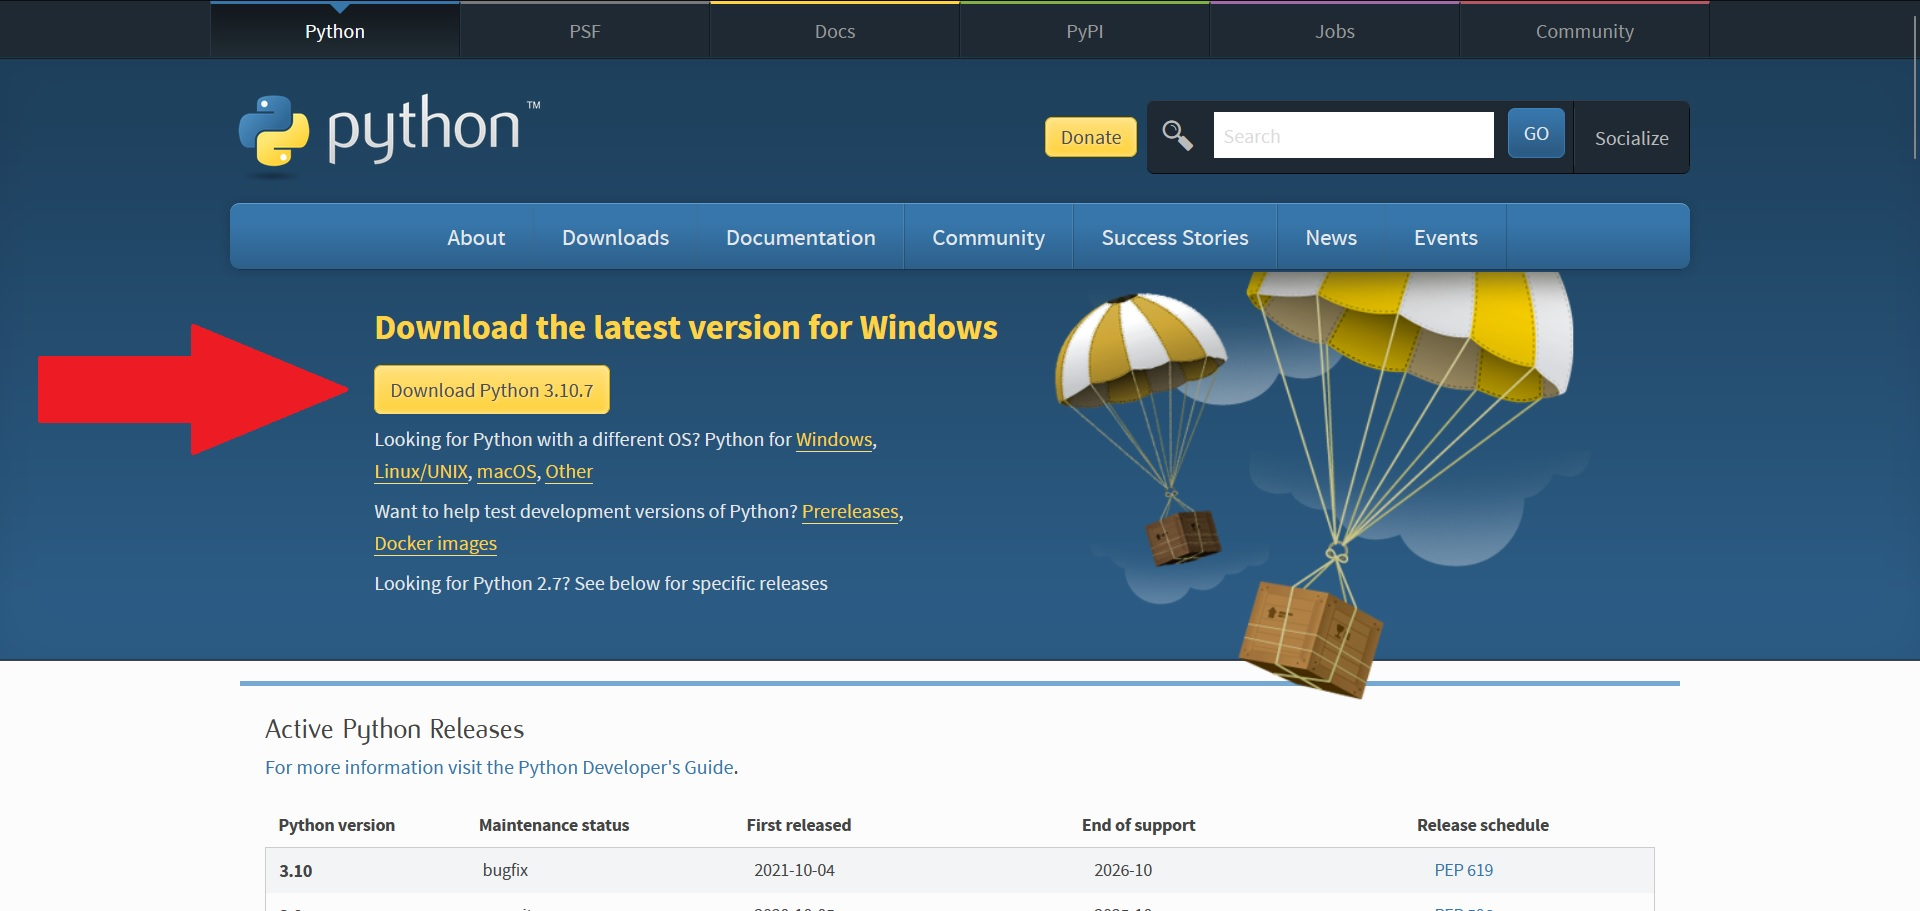
\includegraphics[width=1.0\textwidth]{figures/1.jpg}
    \caption
	{}
    \label{fig:fig1}
\end{figure}

\subsection{مرحله‌ی 2: اجرای نصب‌کننده‌ی \lr{Python}}
پس از دانلود نصب کننده، نصب کننده پایتون را اجرا کنید. مطابق شکل زیر تیک \lr{Install launcher for all users} و \lr{Add Python *.* to PATH} را علامت بزنید. روی \lr{Customize installation} کلیک کنید و سپس روی \lr{Next} کلیک کنید.
\begin{figure}[H]
    \centering
    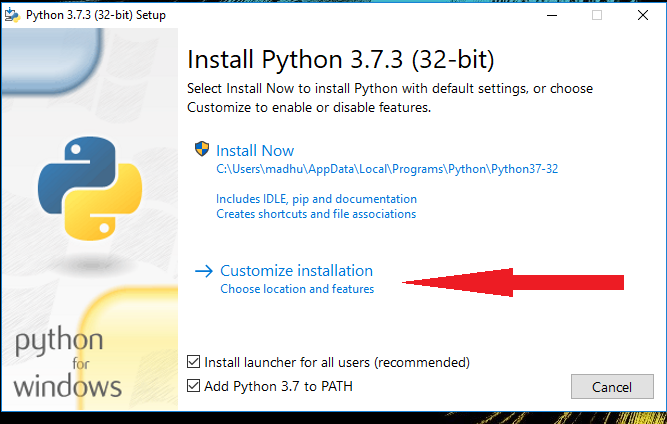
\includegraphics[width=1.0\textwidth]{figures/2.png}
    \caption
	{}
    \label{fig:fig1}
\end{figure}
در صفحه‌ی بعد مطابق شکل 3، تیک تمام گزینه‌ها را بزنید و سپس روی \lr{Next} کلیک کنید.
\begin{figure}[H]
    \centering
    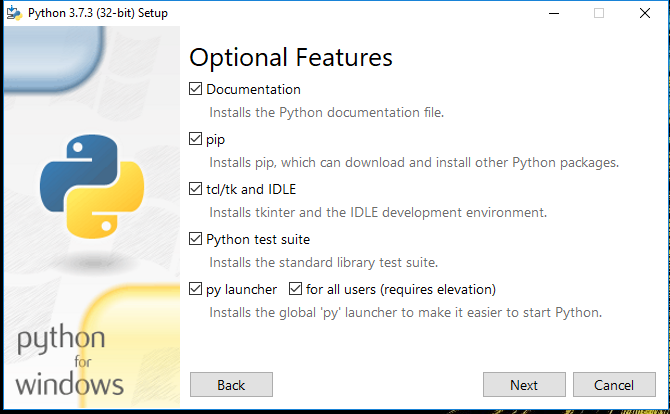
\includegraphics[width=1.0\textwidth]{figures/3.png}
    \caption
	{}
    \label{fig:fig1}
\end{figure}
مطابق شکل 4، تیک گزینه‌های اول تا چهارم (به ویژه گزینه‌ی \lr{Add Python to environment variable} را بزنید) و سپس روی \lr{Install} کلیک کنید.
\begin{figure}[H]
    \centering
    
\includegraphics[width=1.0\textwidth]{figures/4.png}
    \caption
	{}
    \label{fig:fig1}
\end{figure}
پس از اتمام نصب، پنجره‌ی نصب موفق \lr{Python} را مطابق شکل زیر مشاهده خواهید کرد. در نهایت (برای رفع محدودیت 260 کاراکتری مسیرها) روی گزینه \lr{Disable path length limit} کلیک کنید.
\begin{figure}[H]
    \centering
    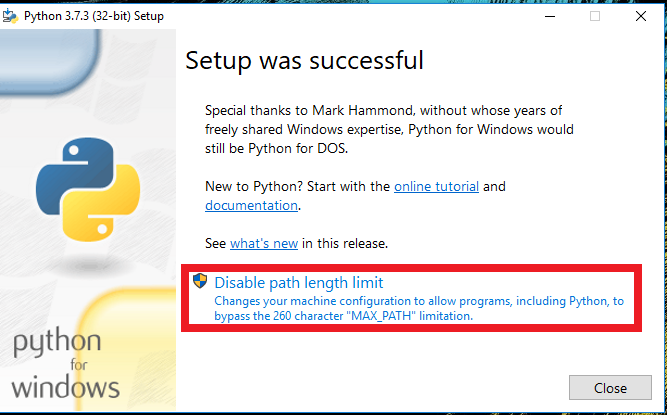
\includegraphics[width=1.0\textwidth]{figures/5.png}
    \caption
	{}
    \label{fig:fig1}
\end{figure}

\subsection{مرحله‌ی 3: اطلاع از صحت نصب \lr{Python}}
اکنون پایتون را با موفقیت در ویندوز نصب کرده‌اید. می‌توانید از طریق خط فرمان (\lr{Command Prompt}) از صحت نصب \lr{Python} اطمینان کسب کنید. \lr{"cmd"} را جستجو کنید و \lr{python} یا \lr{python3} را مطابق شکل تایپ کنید. می بینید که پایتون با موفقیت نصب شده است.
\begin{figure}[H]
    \centering
    
\includegraphics[width=1.0\textwidth]{figures/6.png}
    \caption
	{}
    \label{fig:fig1}
\end{figure}

\section{نصب و پیکربندی \lr{Jupyter Notebook}}
\lr{pip} یک سیستم مدیریت بسته (\lr{package manager}) است که برای نصب و مدیریت بسته‌ها/کتابخانه‌های نرم‌افزاری نوشته شده در پایتون استفاده می‌شود. این فایل‌ها در یک «مخزن آنلاین» بزرگ به نام «شاخص بسته پایتون (\lr{Python Package Index})» (\lr{PyPI}) ذخیره می‌شوند.
\lr{pip} از \lr{PyPI} به عنوان منبع پیش فرض بسته‌ها و وابستگی‌های آن‌ها استفاده می‌کند. برای نصب \lr{Jupyter} با استفاده از \lr{pip}، ابتدا باید بررسی کنیم که آیا \lr{pip} در سیستم ما به روز شده است یا خیر. برای آپدیت \lr{pip} از دستور زیر استفاده کنید:
\begin{latin}
\begin{lstlisting}[language=Python]
python -m pip install --upgrade pip
\end{lstlisting}
\end{latin}
\begin{figure}[H]
    \centering
    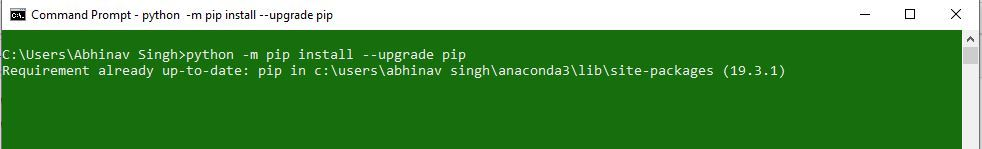
\includegraphics[width=1.0\textwidth]{figures/7.jpg}
    \caption
	{}
    \label{fig:fig1}
\end{figure}
پس از به روز رسانی نسخه‌ی \lr{pip}، دستور زیر را برای نصب \lr{Jupyter} فراخوانی کنید:
\begin{latin}
\begin{lstlisting}[language=Python]
python -m pip install jupyter
\end{lstlisting}
\end{latin}

\begin{figure}[H]
    \centering
    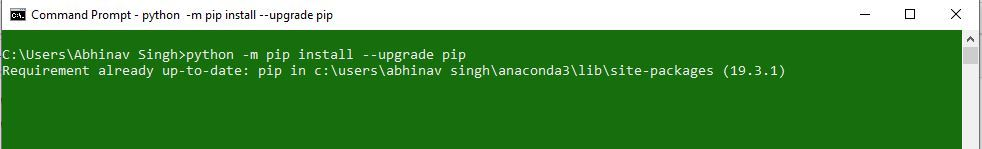
\includegraphics[width=1.0\textwidth]{figures/7.jpg}
    \caption
	{}
    \label{fig:fig1}
\end{figure}
\begin{figure}[H]
    \centering
    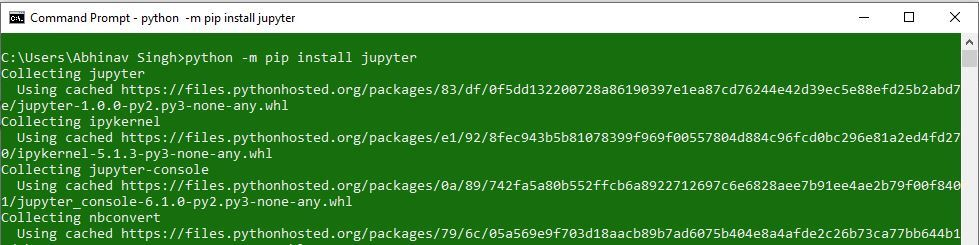
\includegraphics[width=1.0\textwidth]{figures/8.jpg}
    \caption
	{شروع نصب}
    \label{fig:fig1}
\end{figure}
\begin{figure}[H]
    \centering
    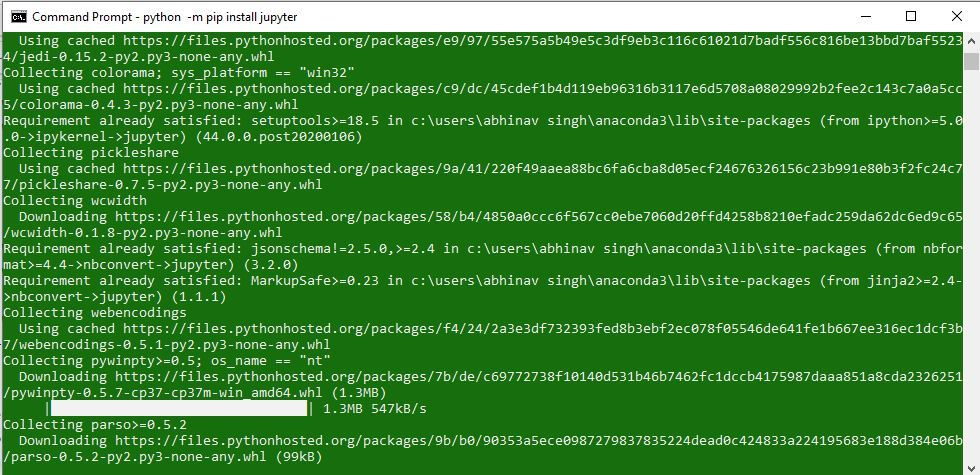
\includegraphics[width=1.0\textwidth]{figures/9.jpg}
    \caption
	{دانلود فایل‌ها و داده‌ها}
    \label{fig:fig1}
\end{figure}
\begin{figure}[H]
    \centering
    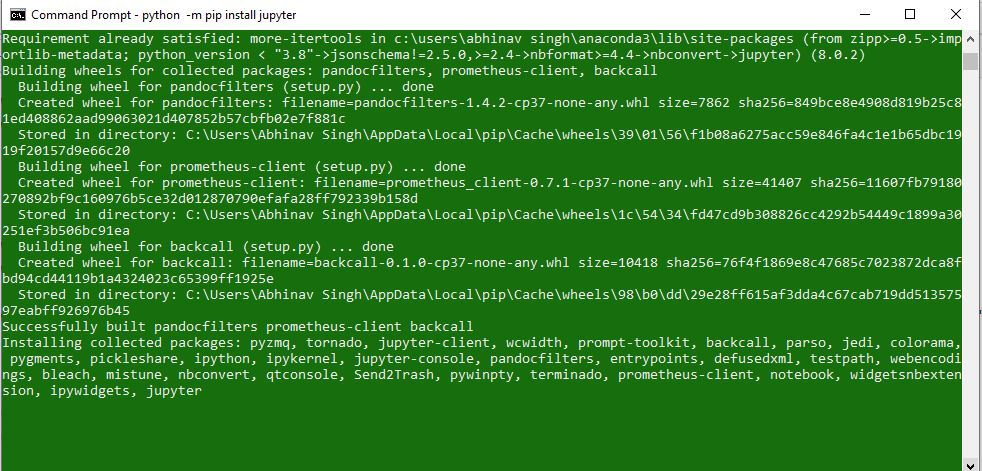
\includegraphics[width=1.0\textwidth]{figures/10.jpg}
    \caption
	{نصب بسته‌ها}
    \label{fig:fig1}
\end{figure}
\begin{figure}[H]
    \centering
    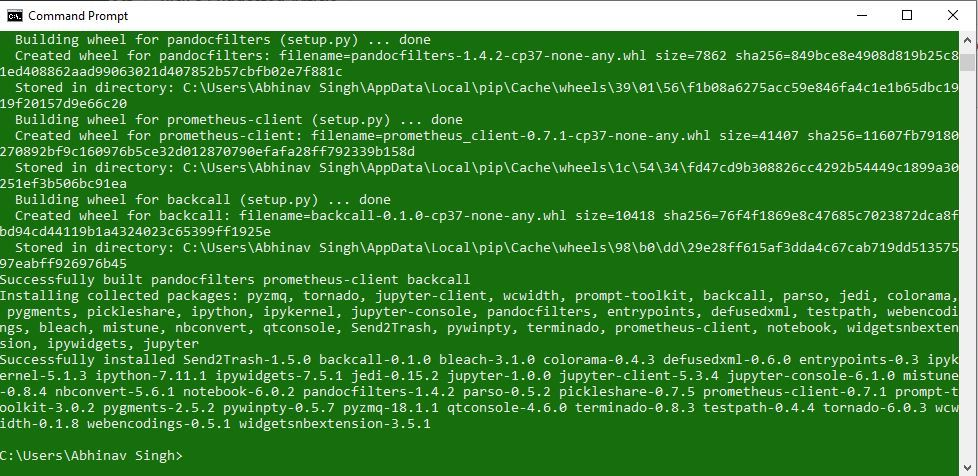
\includegraphics[width=1.0\textwidth]{figures/11.jpg}
    \caption
	{پایان نصب}
    \label{fig:fig1}
\end{figure}

در نهایت از دستور زیر برای راه‌اندازی \lr{Jupyter} با استفاده از خط فرمان استفاده کنید:
\begin{latin}
\begin{lstlisting}[language=Python]
jupyter notebook
\end{lstlisting}
\end{latin}

\begin{figure}[H]
    \centering
    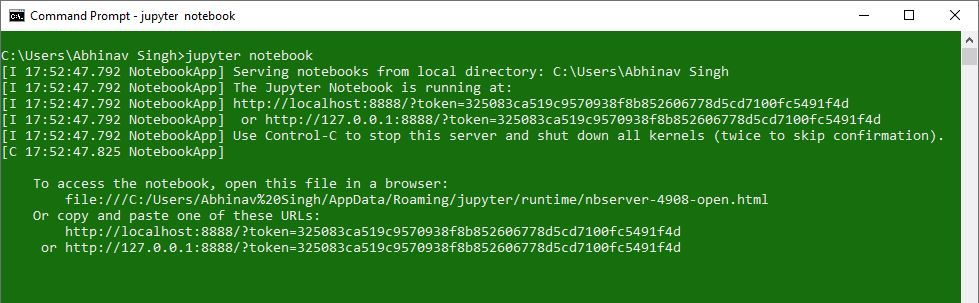
\includegraphics[width=1.0\textwidth]{figures/12.jpg}
    \caption
	{اجرای \lr{Jupyter}}
    \label{fig:fig1}
\end{figure}
\begin{figure}[H]
    \centering
    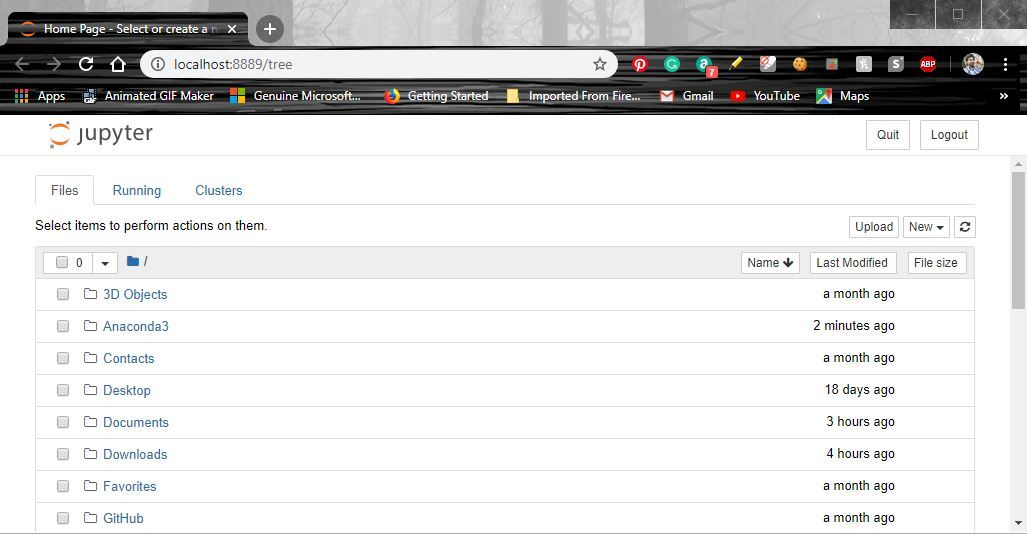
\includegraphics[width=1.0\textwidth]{figures/13.jpg}
    \caption
	{محیط \lr{Jupyter}}
    \label{fig:fig1}
\end{figure}
%%%%%%%%%%%%%%%%%%%%%%%%%%%%%%%%%%%
%%%%%%%%%%%%%%%%%%%%%%%%%%%%%%%%%%%
%%%%%%%%%%%%%%%%%%%%%%%%%%%%%%%%%%%

\section*{منابع}
\renewcommand{\section}[2]{}%
\begin{thebibliography}{99} % assumes less than 100 references
%چنانچه مرجع فارسی نیز داشته باشید باید دستور فوق را فعال کنید و مراجع فارسی خود را بعد از این دستور وارد کنید


\begin{LTRitems}

\resetlatinfont

\bibitem{b1}https://www.digitalocean.com/community/tutorials/install-python-windows-10
\bibitem{b1}https://phoenixnap.com/kb/how-to-install-python-3-windows
\bibitem{b1}https://www.geeksforgeeks.org/how-to-install-jupyter-notebook-in-windows/

\end{LTRitems}

\end{thebibliography}


\end{document}
